
\begin{figure*}
  \centering
  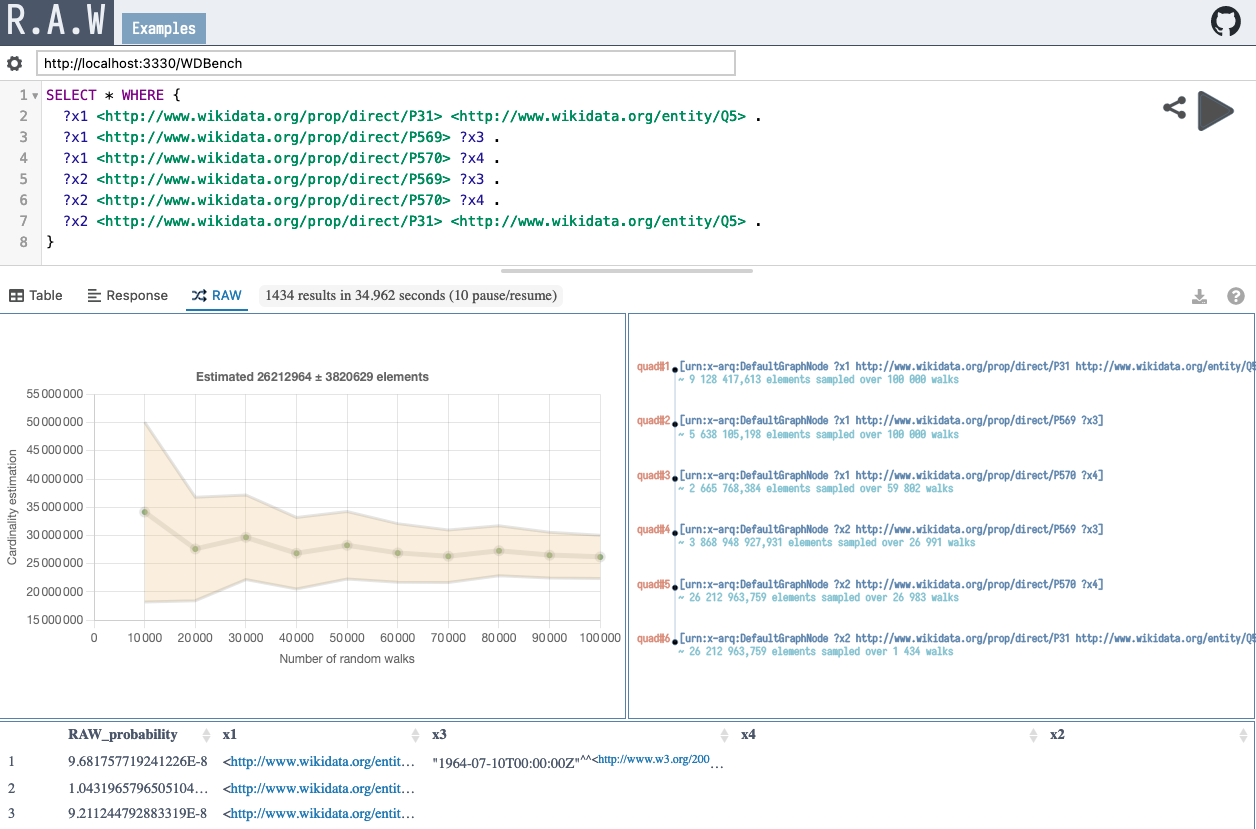
\includegraphics[width=0.85\textwidth]{figures/raw_screenshot.png}
  \caption{\label{fig:raw_screenshot}User interface of \NAME providing useful insights on the query.}
\end{figure*}


 \section{\NAME}
 

 
 As a motivating example, we rely on the query 604 of
 WDbench\cite{angles2022wdbench} presented in the
 figure~\ref{fig:raw_screenshot}. This query are looking for people
 with the same birth and death date. This query returns ~25M results,
 time-out on the public Wikidata SPARQL endpoint, and takes more than
 2 hours to execute on JENA. However, using \NAME, in 35 seconds, it
 is possible to estimate that the query should return around 26
 millions of results more or less 3 millions and return 1434 random
 results

% =======
% \NAME relies on random walks as described in Wander
% Join~\cite{li2019wanderjoin}. Random walks offer several advantages:
% \begin{inparaenum}[(1)]
%   \item They proved to be the best approach for estimating the cardinality
%     of conjunctive SPARQL queries~\cite{park2020g}
%   \item They do not require maintaining statistics~\cite{gubichev2015query}
%   \item They can be efficiently implemented just by relying on
%     traditional SPO, POS, and OSP indexes that are widely available on
%     existing triple stores~\cite{DBLP:conf/cidr/LeisRGK017}.
% \end{inparaenum}
% >>>>>>> 5231642086fb5dee8bbaf39175f7b5ce28485db4

 
To achieve such result,  \NAME first determines a join order for the
query 604 as presented in the figure~\ref{fig:raw_screenshot} on the
right panel with \verb+quad\#1+ to \verb+quad\#6+ 

 
 
% Figure~\ref{fig:raw_screenshot} presents the user interface exploiting
% \NAME's random walks. The top part of the figure shows where the users
% type their queries.

By pressing the play button, \NAME asks the server for random walks on
this whole BGP using the join order described on the right panel of
figure~\ref{fig:raw_screenshot}~\footnote{$quad_1$ to  $quad_6$ }. When the server reaches a configurable threshold
of $10 000$ random walks, or $60s$ execution time, it returns its
results.

Random walks follow the join order for $Q_{604}$. Starting from the
\verb+quad\#1+, it draws a random mapping $\mu_1$ for \verb+?x1+ with
a probability of $1/|quad_1|$. As \verb+?x1+ is now bounded, it draws a
random mapping $\mu_2$ for \verb+?x3+ for the second triple pattern
with a probability of $1/|mu_1@quad_2|$. with $\mu_1$ and $\mu_2$, the
random walk cannot find a result for the third triple pattern
$quad_3$. The random walk failed but is returned along with the
probability of this path as described in the lower panel of the
figure~\ref{fig:raw_screenshot}.

By collecting 10000 walks like this in 2s, \NAME is able to compute
the first cardinality estimation in the left panel of
figure~\ref{fig:raw_screenshot} ie. it estimates the cardinality of
the query to 34M more or less 15M. It also display estimated
cardinalities for each triple pattern of the join order in the right panel.

By repeating the operation, results are
merged iteratively in a pay-as-you-go fashion hence displaying more
accurate information. Figure~\ref{fig:raw_screenshot} shows that over
$10$ iterations, \NAME performed $100k$ random walks but only $1434$
actual successes.  Yet, the bottom left figure provides an estimation
of the number of results over the number of random walks with
confidence intervals. The bottom right figure provides the estimated
number of intermediate results along with the number of random walks
that reached each triple/quad pattern.  Finally, the bottom part shows
both failed and succeeded random walks along with the probability that
they were chosen at execution time.

 
 
%
%\begin{figure}[t]
%   \centering
%   \begin{minipage}{0.49\textwidth}
%     \subfloat[$(Q_e$]{
%       \lstinputlisting[
%         basicstyle=\scriptsize\sffamily,
%         language=sparql,
%         numbers=none,
%         columns=fixed,
%         showstringspaces=false]{
%           figures/query-q1-j2-no-star.rq
%         }
%       \label{fig:q1-j2-1hop}
%     } \\
%     % \subfloat[$(Q_1^{J_2})^{1..2}$]{
%     %   \lstinputlisting[
%     %     basicstyle=\scriptsize\sffamily,
%     %     language=sparql,
%     %     numbers=none,
%     %     columns=fixed,
%     %     showstringspaces=false]{
%     %       figures/query-q1-j2-2hop.rq
%     %     }
%     %   \label{fig:q1-j2-2hop}
%     % }
%   \end{minipage}
%   \hfill
%   \begin{minipage}{0.50\textwidth}
%     \subfloat[RDF graph $G_1$]{
%       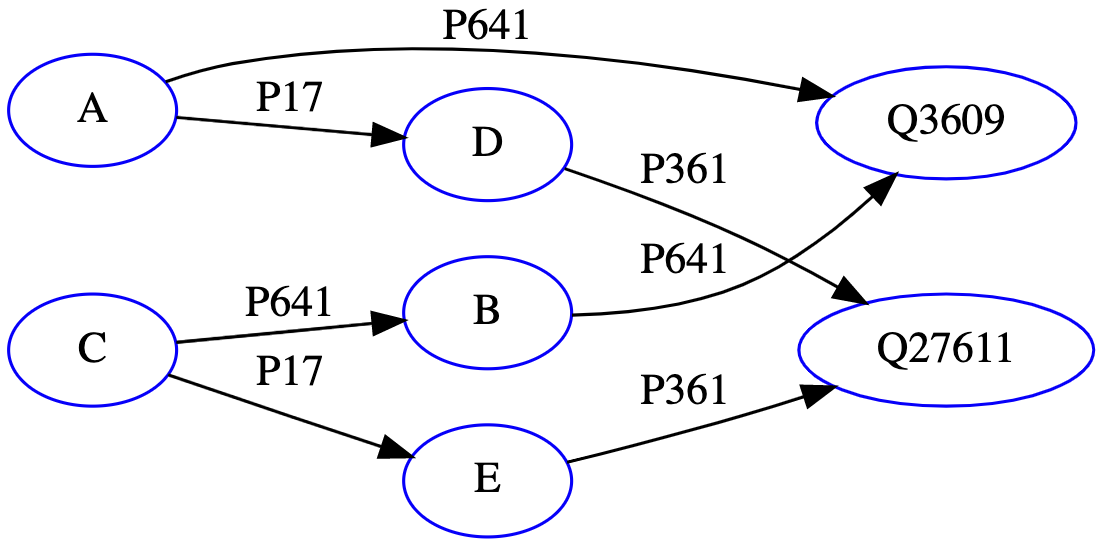
\includegraphics[width=\textwidth]{figures/graph-g1.png}
%     }
%   \end{minipage}
%   \caption{
%     query $Q_e$  evaluated on RDF graph $G_1$.
%   }
%   \label{fig:random_walks_example}
% \end{figure}



% \section{\NAME}

% \NAME relies on random walks as described in
% WanderJoin\cite{li2016wanderjoin}. Random
% walks~\cite{DBLP:journals/tods/LiWYZ19} offer several advantages:
% \begin{inparaenum}[(1)]
%   \item They proved to be the best approach for estimating the cardinality
%     of conjunctive SPARQL queries~\cite{park2020g}
%   \item They do not require maintaining statistics~\cite{gubichev2015query}
%   \item They can be efficiently implemented just by relying on
%     traditional SPO, POS, and OSP indexes that are widely available on
%     existing triple stores~\cite{DBLP:conf/cidr/LeisRGK017}.
% \end{inparaenum}


% Let $Q$ be a SPARQL conjunctive query, and $J = \langle tp_1, ..., tp_n \rangle$ be
% the join order used to perform random walks. A random walk
% $\gamma_i = \langle t_1, ..., t_n\rangle$ is computed over
% an RDF graph $G$ by randomly picking $t_1$ in $\llbracket tp_1 \rrbracket_G$,
% and each subsequent $t_i$ ($i > 1$) in $\llbracket t_{i-1} \bowtie tp_i \rrbracket_G$.
% Once computed, the cardinality of $Q$ is estimated as the inverse probability
% of sampling $\gamma_i$, i.e. $P(\gamma_i)^{-1}$, with $P(\gamma_i) = |\llbracket tp_1 \rrbracket_G|^{-1} \prod_{i=2}^{n}
% |\llbracket t_{i-1} \bowtie tp_i \rrbracket_G|^{-1}$.

% For instance, let us consider the query $Q_e$ and the RDF graph $G_1$
% depicted in Figure~\ref{fig:random_walks_example}. Following the join order $tp_3,tp_2,tp_1$, the random walk 
% $\gamma_1$ is computed as follow:

% % \begin{center}
%   \begin{small}
%     \begin{tabular}{l|lll}
%       $tp_3$ & draw  $t_1$ &$= (\textbf{A}, P641, Q3609)$ & $\in \llbracket (?x1, P641, Q3609) \rrbracket_{G_1}$ \\
%       $tp_2$ & draw  $t_2$ &$= (A, P17, \textbf{D})$ & $ \in \llbracket (\textbf{A}, P17, ?x3) \rrbracket_{G_1}$  \\
%       $tp_1$ & draw  $t_3$ &$= (D, P361, Q27611)$ & $\in \llbracket (\textbf{D}, P361, Q27611) \rrbracket_{G_1}$  
%     \end{tabular}
%   \end{small} 
% % \end{center}

% \noindent The cardinality of $Q_e$ is then estimated as the inverse
% probability of sampling $\gamma_1$:
% \begin{small}

% \noindent\begin{tabular}{ll}
%     $P(\gamma_1)^{-1}$  &$=  |\llbracket (?x1, P641, Q3609) \rrbracket_{G_1}| \times
%                           |\llbracket (\textbf{A}, P17, ?x3) \rrbracket_{G_1}| \times
%                           |\llbracket (\textbf{D}, P361,
%                           Q27611) \rrbracket_{G_1}| $ \\
%                       &$=  2 \times 1 \times 1 = 2$
% \end{tabular}
% \end{small}

% \noindent Of course, a random walk may fail if it becomes impossible to sample $t_i$ for
% some $i \leq n$. In this case, its probability $P(\gamma_i)$ of being sampled is 0.
% For instance, if $t_1 = (B, P641, Q3609)$ is picked in
% $\llbracket (?x1, P641, Q3609) \rrbracket_{G_1}$
% instead of $(A, P641, Q3609)$, then the random walk fails because
% $\llbracket (B, P17, ?x3) \rrbracket_{G_1} = \emptyset$.
% %
% To improve the quality of estimates, instead of computing only one random
% walk, a set $\Gamma = \langle \gamma_1, ..., \gamma_k \rangle$ of $k$ random walks is computed,
% and the cardinality of the query is estimated as $card(\Gamma) = |\Gamma|^{-1}\sum_{i=1}^{|\Gamma|} P(\gamma_i)^{-1}$.

% In \NAME, we implemented random walks using B-Trees of JENA. Under
% Sampling a query returns the random walk performed during query
% execution along with cardinality estimation. 

% %  \begin{figure}[t]
% %   \begin{center}
% %    \subfloat [Query $Q_1^{J_1}$ time-out >60s] {\label{fig:q1-nojo}
% %     \adjustbox{valign=T}{
% %     \resizebox{0.45\textwidth}{!}{
% %      \lstinputlisting[basicstyle=\scriptsize\sffamily,
% %      language=sparql,numbers=none,columns=fixed,
% %      showstringspaces=false]{./figures/q1w.rq}}}}
% %   \subfloat [Query $Q_1^{J_2}$ forced join order $\sim 451ms$] {\label{fig:q1j2}
% %    \adjustbox{valign=T}{
% %     \resizebox{0.45\textwidth}{!}{
% %      \lstinputlisting[basicstyle=\scriptsize\sffamily,
% %      language=sparql,numbers=none,columns=fixed,
% %      showstringspaces=false]{./figures/q1w-jo.rq}}}}
% %  \end{center}
% %  \caption{The query $Q_1$ searches for creative works and the list of
% %   fiction works that inspired them. $Q_1$ time-out on
% %   the Wikidata online server (>60s)}
% %  \label{fig:q1}
% % \end{figure}


% Pay-as-you-go \texttt{:)}.

% The more the server can do, the better. But client must also be able
% to process and merge incoming control information.

% We enhanced Apache Jena with random walks over its default internal
% storage called TDB2.


% %%% Local Variables:
% %%% mode: latex
% %%% TeX-master: "../paper.tex"
% %%% End:
